\section{Implementation and Reproducibility}
The two studies used the existing repository generators, constraint parsing, VCG circuits, and PenaltyQAOA implementation through the tuning scripts. Computation used PennyLane 0.43.1 with the \texttt{default.qubit} simulator, JAX/JAXlib 0.6.2, Optax 0.2.5, NumPy 2.2.6, and Python 3.13.13, with 64-bit CPU arithmetic. The dataset seed was 42, the training seed root was 7, and the sampling seed root was 19. Stable hashes of instance and phase identifiers derived the optimization seeds. Penalty-setting identifiers additionally entered the sampling seeds. No complete training-seed replication was performed.

Tasks were grouped by constraint or COP to reuse circuit preparation and compiled functions across conditions. Standard-QAOA penalty circuits combined repeated commuting Pauli terms before compilation while retaining separate numerical objective and penalty weights. The shared angle permits this combination without changing the ideal circuit, apart from irrelevant identity phases. VCG circuits retained the existing ma-QAOA parameter layout. Optimization checkpoints stored angles, Adam state, random state and progress every ten steps and at restart, depth and task boundaries. Files were written atomically with a previous-checkpoint backup.

The default allocation was two workers with six physical CPU cores per worker. Accumulated compile/warm-up time was approximately 10.87 worker-hours for Study A and 0.57 worker-hours for Study B; synchronized optimizer-update time was approximately 10.22 and 14.18 worker-hours, respectively. These totals are sums across tasks, not elapsed wall time, and exclude some I/O and analysis costs. Compilation counters include disposable warm-up calls and overhead on reused functions. The largest recorded worker RSS was approximately 14.54 GiB in Study A and 14.82 GiB in Study B. A worker's RSS is a process high-water mark, not a per-task allocation.

PenaltyQAOA used 4--19 total qubits, including 0--12 slack qubits. Figure~\ref{cal:resources} shows the measured simulation times and qubit counts. The displayed PC-QAOA slack counts are computed partitions only; no PC-QAOA simulation is included.

\begin{figure}[tb]
\centering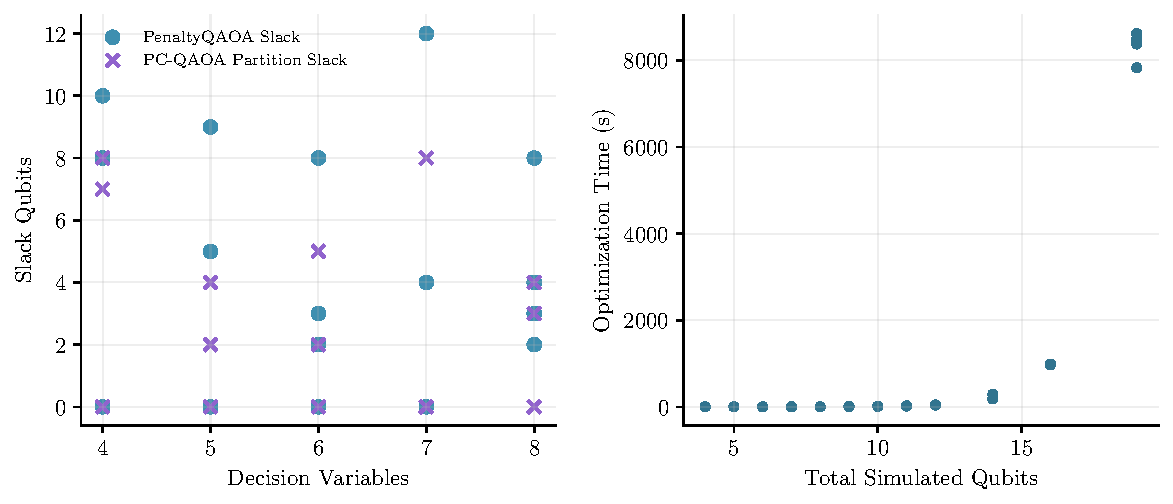
\includegraphics[width=0.9\linewidth]{figures/b_qubits_runtime.pdf}
\caption{Decision/slack counts and recorded PenaltyQAOA optimizer-update times. Each runtime point is a completed instance--method task across depths one through five. The PC-QAOA points represent hypothetical partition slack counts, not measured PC-QAOA execution.}
\label{cal:resources}
\end{figure}

\paragraph{Archived evidence.}
The report's \texttt{data/} directory contains copies of the original run records, manifests and selected-setting records, along with per-task summaries, ranking tables, and paired comparisons. The copied run records preserve source-file hashes, base commit and package versions. Study A and Study B have separate run identifiers because Study B was revised after Study A began. The obsolete multiplier configuration in Study A's run record was not used for the reported Study B results; the separate Study B record specifies the five fixed methods. The report generation record also hashes the analysis source used to produce its tables and figures.

The selected VCG database contains one gadget per calibration constraint trained with $L_{\mathrm{fid}}$. It remains in the original results directory. The report summarizes saved final results and does not modify selections, checkpoints, gadget states or optimizer histories.

\section{Additional Diagnostic Figures}
\begin{figure}[tb]
\centering
\begin{subfigure}{0.49\linewidth}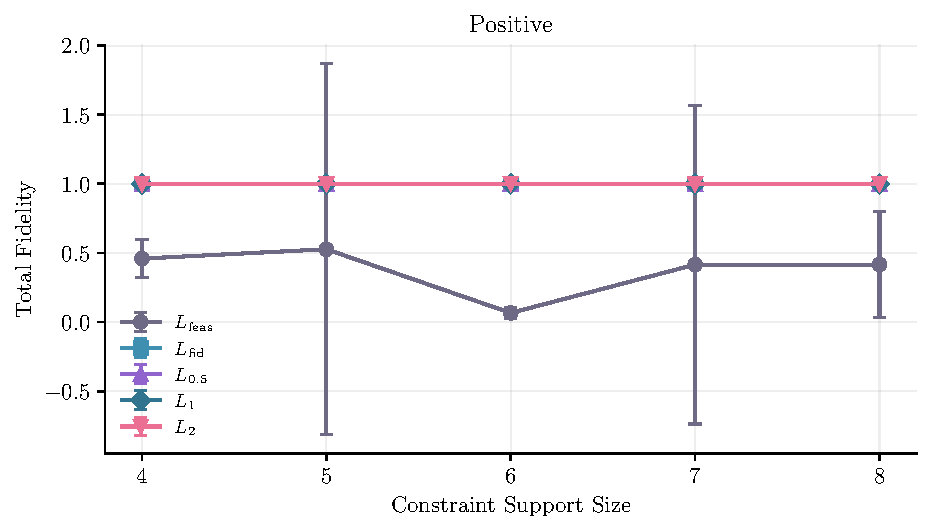
\includegraphics[width=\linewidth]{figures/a_fidelity_positive.pdf}\caption{Positive weighted inequalities.}\end{subfigure}\hfill
\begin{subfigure}{0.49\linewidth}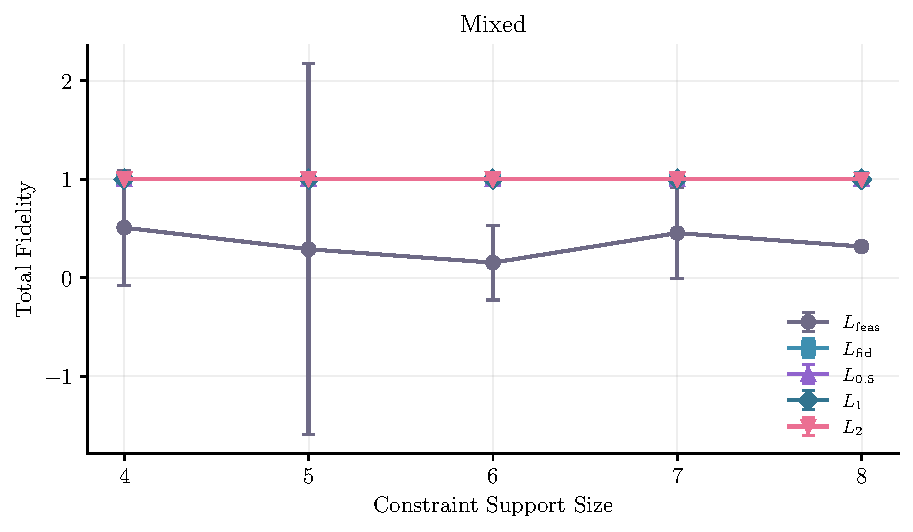
\includegraphics[width=\linewidth]{figures/a_fidelity_mixed.pdf}\caption{Mixed-sign inequalities.}\end{subfigure}\\
\begin{subfigure}{0.49\linewidth}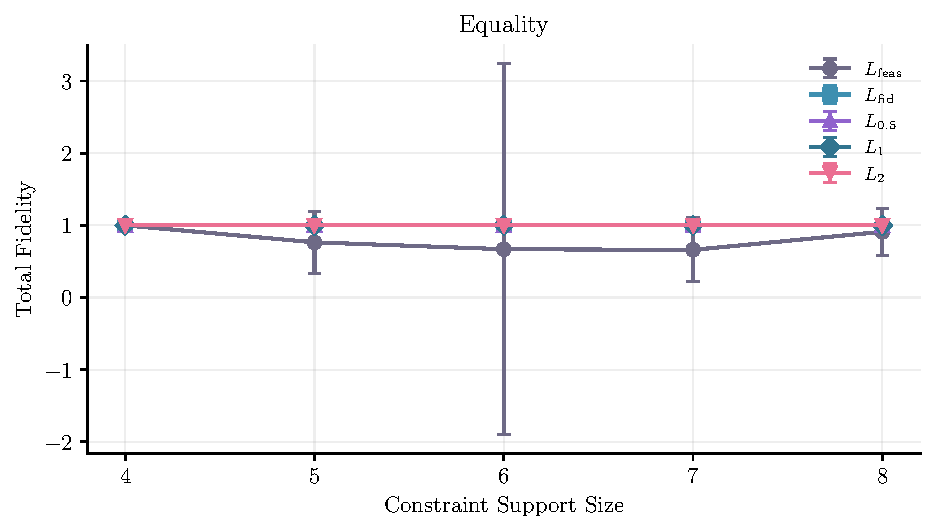
\includegraphics[width=\linewidth]{figures/a_fidelity_equality.pdf}\caption{Weighted equalities.}\end{subfigure}\hfill
\begin{subfigure}{0.49\linewidth}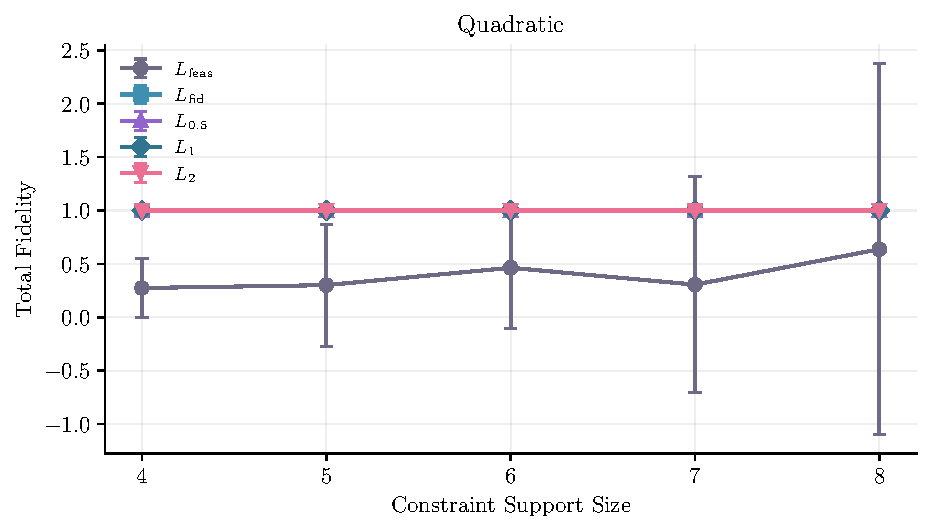
\includegraphics[width=\linewidth]{figures/a_fidelity_quadratic.pdf}\caption{Quadratic inequalities.}\end{subfigure}
\caption{Returned VCG fidelity by family and support size. Each point contains two or three constraints. The pointwise $t$ intervals can be wide or extend beyond physical probability bounds because of the small groups.}
\end{figure}
\begin{figure}[tb]
\centering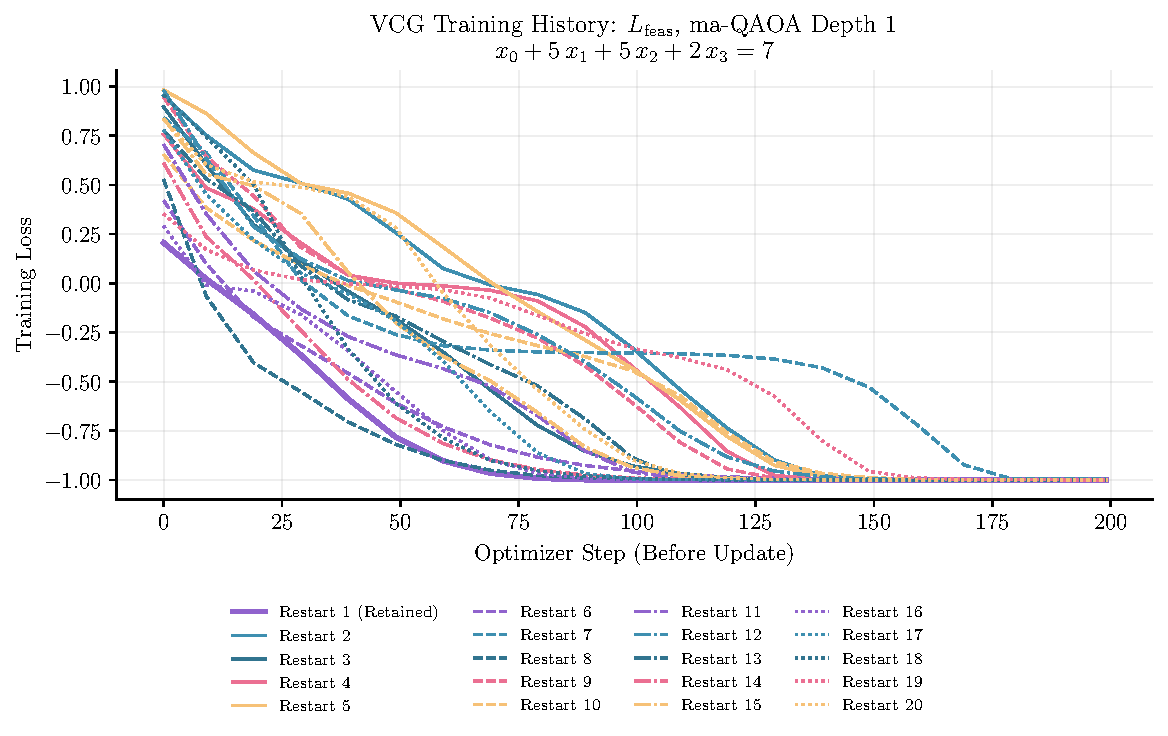
\includegraphics[width=0.8\linewidth]{figures/a_training_history.pdf}
\caption{Example VCG training histories. The title identifies the constraint, loss and depth. Each curve is one restart; the retained restart has the lowest final training loss. The plotted loss is evaluated before the indicated update, whereas restart selection uses the loss after the final update. Loss approaching $-1$ under $L_{\mathrm{feas}}$ indicates feasible probability approaching one, not necessarily uniform-state fidelity approaching one.}
\end{figure}
\begin{figure}[tb]
\centering
\begin{subfigure}{0.49\linewidth}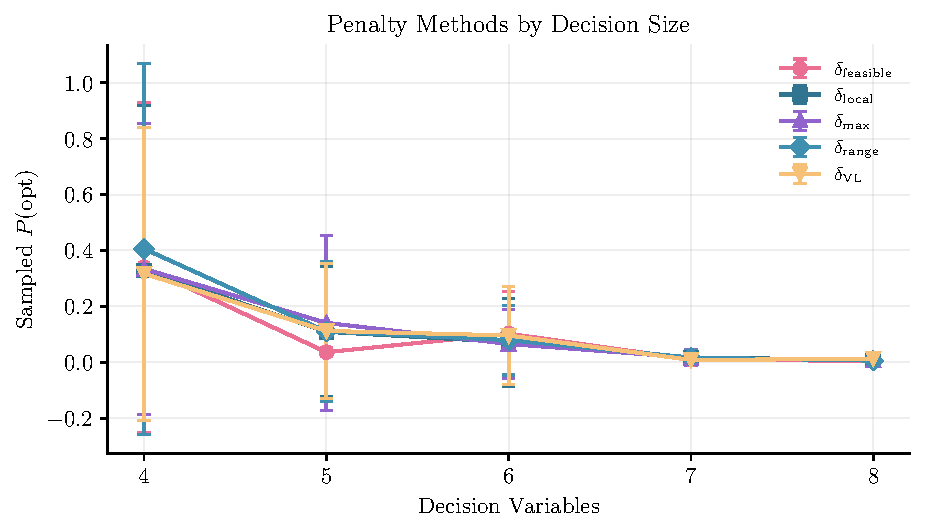
\includegraphics[width=\linewidth]{figures/b_sizes.pdf}\caption{Size dependence.}\end{subfigure}\hfill
\begin{subfigure}{0.49\linewidth}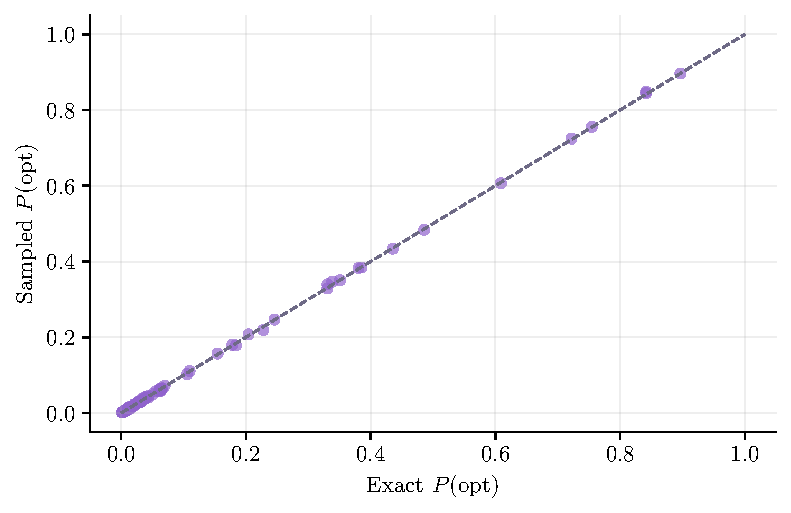
\includegraphics[width=\linewidth]{figures/b_sampled_exact.pdf}\caption{Sampled and exact probabilities.}\end{subfigure}
\caption{Study B diagnostics. Left: means over four COPs per decision size, with pointwise 95\% intervals. Right: exact and sampled depth-five success probabilities for all 100 tasks. The diagonal denotes equality; exact values do not enter penalty selection.}
\end{figure}
\FloatBarrier
